\documentclass{standalone}
\usepackage{tikz}

\usetikzlibrary{calc}


\begin{document}

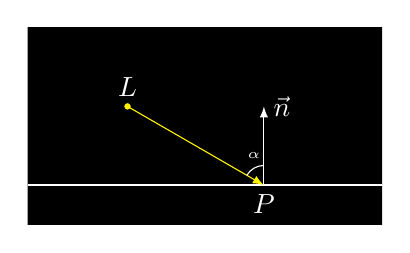
\begin{tikzpicture}
  \path[clip] (-1,-0.5) rectangle (3.5,2);
  \draw[fill=black] (-1,-0.5) rectangle (3.5,2);
  \draw[thick,white] (-1,0) -- (4,0);

  \coordinate (hit) at (2,0);
  \coordinate (light) at ($ (hit) + (150:2) $);
  \coordinate (eye) at (3,1.5);

  \draw[fill=yellow] (light) circle [radius=0.05cm] node [white,above] {$L$};
  \draw[yellow,-latex] (light) -- (hit);

  \node[anchor=north,white] at (hit) {$P$};

  \draw[-latex,white] (hit) -- ++(0,1) node[anchor=west] {$\vec n$};

  \draw[white] ($ (hit) + (90:0.25) $) arc [start angle=90,delta angle=60,radius=0.25] node[midway,above,font=\tiny] {$\alpha$};
\end{tikzpicture}

\end{document}